\section{问题四：离网运行及储能配置研究}

\subsection{问题分析}

本问题研究园区离网运行模式，即切断与外部电网的连接，园区用能完全依赖风光发电。在产能72吨/日、功率连续可调（下限10\%）的条件下，需要分析无储能和有储能两种情况下的制氨产量和经济性，并对比离网与联网两种运行模式。

\begin{figure}[H]
\centering
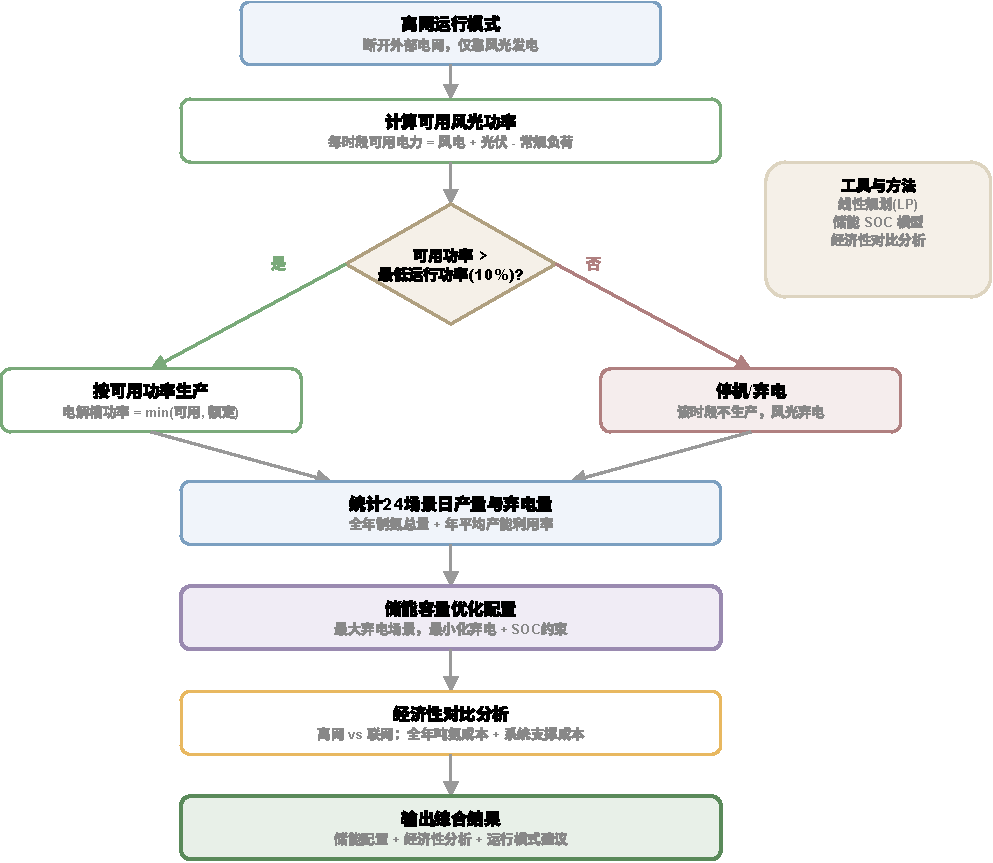
\includegraphics[width=0.85\textwidth,height=0.38\textheight,keepaspectratio]{../figures/fig_flow_q4.pdf}
\caption{问题四求解流程图}\label{fig:flow_q4}
\end{figure}

问题四的求解流程如图\ref{fig:flow_q4}所示，分为三个递进的子问题：无储能离网运行（确定产量上限）、储能配置优化（提升产量和利用率）、离网与联网经济性对比（评估系统支撑价值）。

\subsection{子问题(1)：无储能离网运行}

\subsubsection{模型建立}

离网模式下无外部电网支撑，功率平衡方程变为：
\begin{equation}
P_{wind}(t) + P_{pv}(t) = \alpha(t) \cdot P_{EHA}^{rated} + P_{load}(t) + P_{curtail}(t), \quad \forall t
\end{equation}

其中$P_{curtail}(t) \geq 0$为弃电功率。关键约束为每时段用电不能超过风光发电：
\begin{equation}
\alpha(t) \leq \alpha_{max}(t) = \min\left(\frac{P_{wind}(t) + P_{pv}(t) - P_{load}(t)}{P_{EHA}^{rated}},\ 1.0\right)
\end{equation}

若$\alpha_{max}(t) < 0.1$，则该时段必须停机（$\alpha(t) = 0$）。目标为最大化日产氨量：
\begin{equation}
\max \quad M_{NH3} = 3.0 \sum_{t=1}^{24} \alpha(t) \text{ (吨)}
\end{equation}

由于各时段独立（无时间耦合），最优解为$\alpha^*(t) = \alpha_{max}(t)$（若$\alpha_{max}(t) \geq 0.1$）或$\alpha^*(t) = 0$（否则）。

\subsubsection{求解结果}

\begin{table}[H]
\centering
\caption{离网各场景产量与成本（部分场景）}\label{tab:q4_offgrid}
\resizebox{\textwidth}{!}{
\begin{tabular}{cccccc}
\toprule
场景 & 制氨产量(吨/日) & 吨氨成本(元/吨) & 风光利用率(\%) & 弃电量(MWh) & 发电量(MWh) \\
\midrule
W1P1 & 39.98 & 4143 & 80.6 & 147.9 & 761.8 \\
W1P2 & 30.54 & 3893 & 96.0 & 20.1 & 503.2 \\
W1P3 & 19.09 & 4185 & 96.3 & 12.6 & 337.4 \\
W1P4 & 13.91 & 4565 & 92.8 & 19.7 & 272.8 \\
W2P1 & 36.10 & 3982 & 85.0 & 99.0 & 658.9 \\
W2P2 & 23.88 & 3867 & 97.7 & 9.4 & 400.3 \\
W2P3 & 11.62 & 4477 & 94.4 & 13.3 & 234.6 \\
W2P4 & 6.25 & 5649 & 86.6 & 22.9 & 169.9 \\
W3P1 & 42.92 & 4040 & 83.8 & 126.4 & 780.8 \\
W3P2 & 33.10 & 3807 & 99.3 & 3.7 & 522.3 \\
\bottomrule
\end{tabular}}
\end{table}

离网各场景的产量与成本如表\ref{tab:q4_offgrid}所示。日产量范围为6.2--46.2吨/日，吨氨成本范围为3798--5649元/吨，风光利用率范围为79.8\%--100.0\%。全年总产氨量为9782吨，年平均产能利用率仅为37.7\%，远低于联网模式。

\begin{figure}[H]
\centering
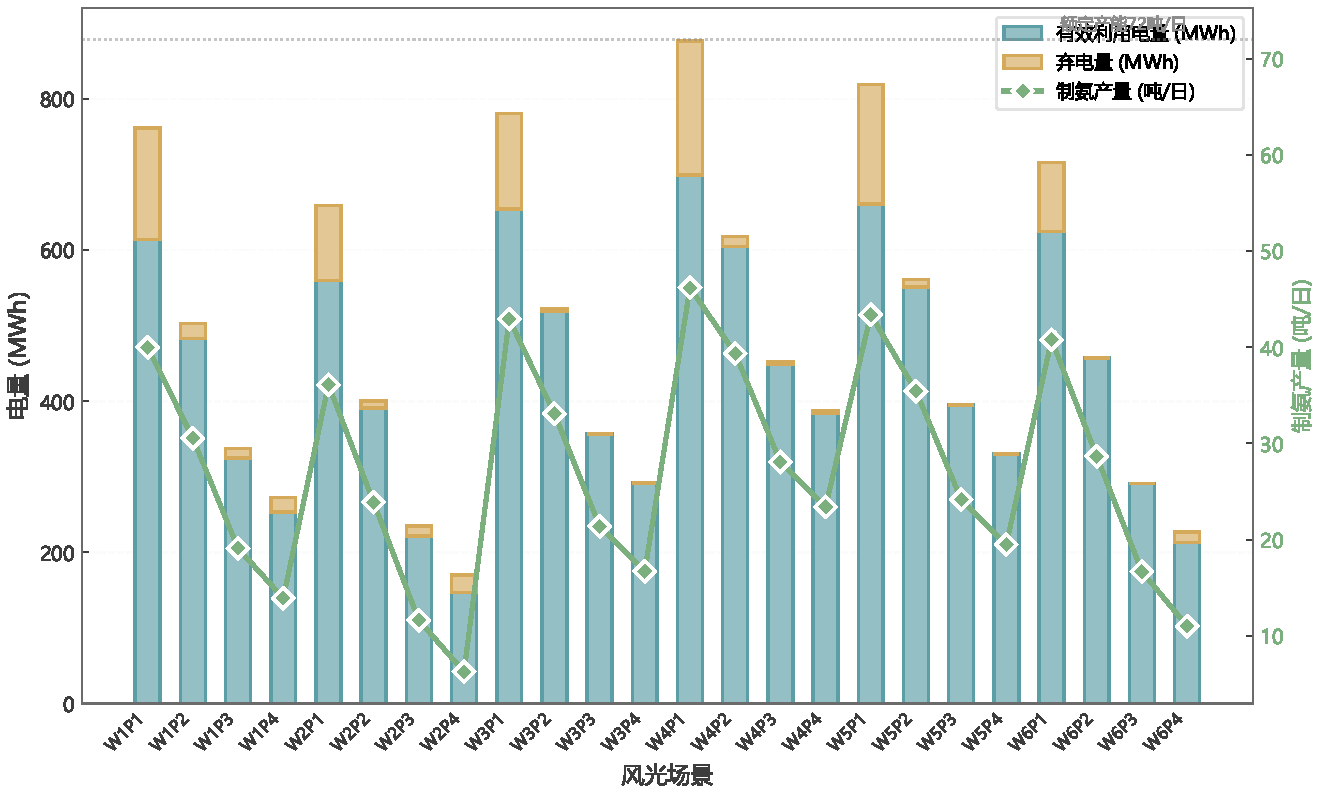
\includegraphics[width=0.85\textwidth,height=0.38\textheight,keepaspectratio]{../figures/fig_q4_offgrid_production.pdf}
\caption{24场景离网产量与电量利用分布}\label{fig:q4_offgrid_production}
\end{figure}

离网产量分布（图\ref{fig:q4_offgrid_production}）呈现明显的两极分化：高风光场景（W3P1、W4P1等）日产量可达40吨以上，而低风光场景（W2P4、W6P4等）日产量不足10吨。这种极端波动性是离网模式的固有缺陷——没有电网的"削峰填谷"功能，产量完全受制于当日风光资源。最大弃电场景为W4P1（弃电177.3 MWh），该场景风光资源极为丰富但设备产能有限，大量电力无法消纳。

最小风光装机容量估算结果为：风电155.0 MW + 光伏0 MW = 155.0 MW，可保证所有场景下至少维持10\%负荷运行。该结果表明，纯风电方案在保障基本运行方面优于风光混合方案，因为风电在夜间仍有出力而光伏完全为零。

\subsection{子问题(2)：储能配置优化}

\subsubsection{模型建立}

针对最大弃电场景W4P1，引入储能系统。储能状态方程为：
\begin{equation}
E_{sto}(t+1) = E_{sto}(t) \cdot (1 - \sigma) + P_{sto,c}(t) \cdot \eta_c \cdot \Delta t - \frac{P_{sto,d}(t)}{\eta_d} \cdot \Delta t   \cite{ref5}
\end{equation}

其中$\eta_c = \eta_d = 0.90$为充放电效率，$\sigma = 0.002$/h为自损耗率。离网功率平衡（有储能）为：
\begin{equation}
P_{wind}(t) + P_{pv}(t) + P_{sto,d}(t) = \alpha(t) \cdot P_{EHA}^{rated} + P_{load}(t) + P_{sto,c}(t) + P_{curtail}(t)
\end{equation}

目标函数为最小化含储能投资的综合吨氨成本。储能单位投资成本设定为$c_{inv} = 1000$元/kWh，项目设计寿命为$Y = 15$年。将储能建设成本等额分摊至单日，构建综合成本目标函数：$$C_{ton}^{sto} = \frac{C_{RE} + C_{OM} + C_{buy} - C_{sell} + C_{sto\_daily}}{M_{target}}$$其中，储能单日折算成本$C_{sto\_daily}$为：
$$C_{sto\_daily} = C_{sto} \times 10^3 \times \frac{c_{inv}}{365 \times Y}$$
模型求解采用两层优化策略：外层运用网格搜索法寻优储能容量$C_{sto}$，内层基于线性规划（LP）求解给定容量下的最优充放电调度方案。

%目标函数为最小化含储能投资的综合吨氨成本，储能投资按1000元/kWh、15年寿命分摊至每日。采用两层优化策略：外层网格搜索最优储能容量$C_{sto}$，内层LP求解给定容量下的最优调度。

\subsubsection{求解结果}

\begin{table}[H]
\centering
\caption{储能配置方案及效果}\label{tab:q4_storage}
\begin{tabular}{lc}
\toprule
参数 & 数值 \\
\midrule
最优储能容量 (MWh) & 5 \\
目标场景 & W4P1 \\
配储后制氨产量 (吨/日) & 46.51 \\
配储后吨氨成本 (元/吨) & 4189.10 \\
全年制氨总量 (吨) & 9831.0 \\
平均产能利用率 & 37.93\% \\
\bottomrule
\end{tabular}
\end{table}

储能配置优化结果如表\ref{tab:q4_storage}所示。最优储能容量为5 MWh，在W4P1场景下可将日产量从39.98吨提升至46.51吨（+16.3\%），吨氨成本从4143元/吨微升至4189元/吨。储能容量增大时产量提升但投资分摊增加，边际效益递减，5 MWh为综合成本最优点。

\begin{figure}[H]
\centering
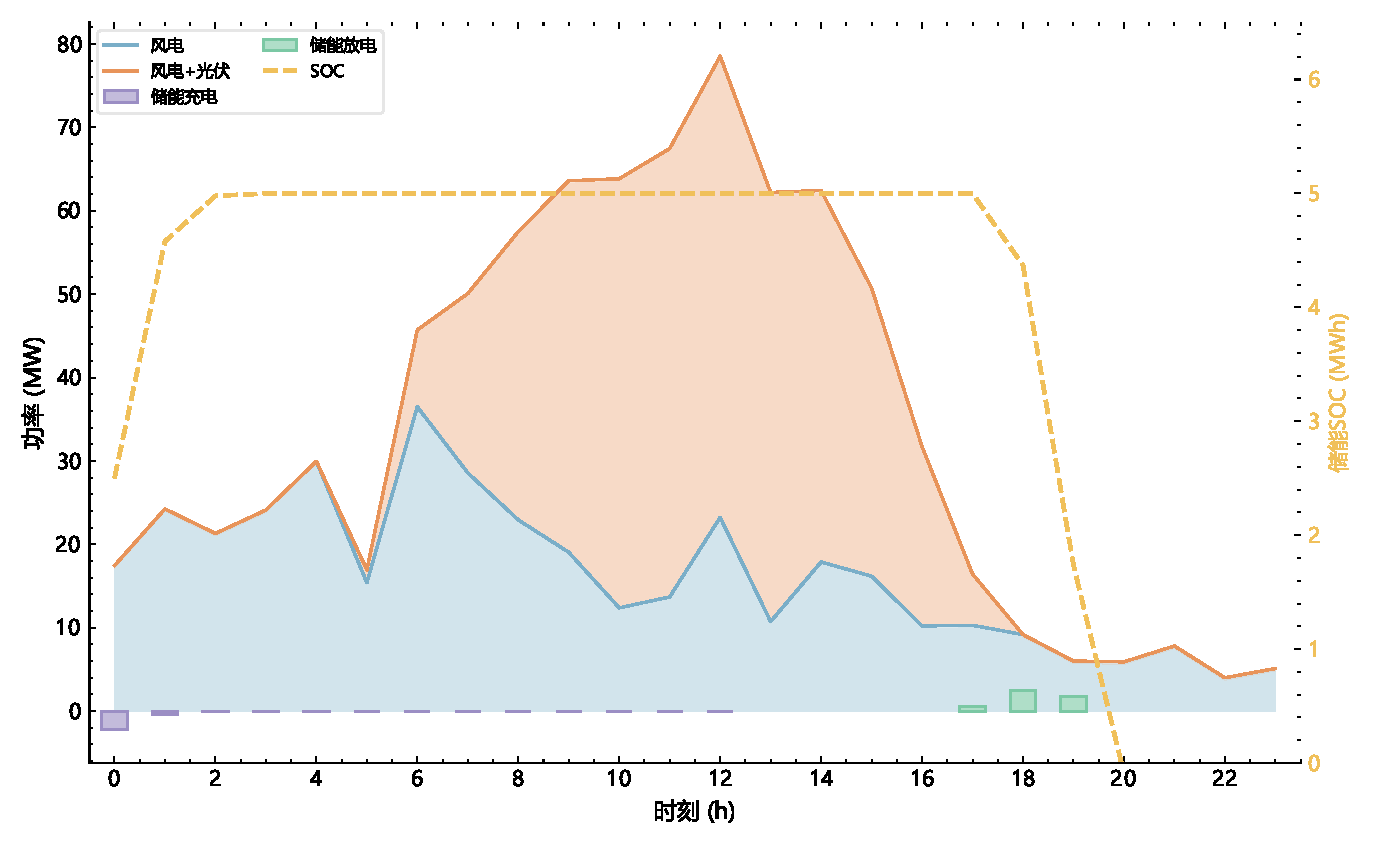
\includegraphics[width=0.85\textwidth,height=0.38\textheight,keepaspectratio]{../figures/fig_q4_storage_dispatch.pdf}
\caption{最大弃电场景储能充放电调度方案}\label{fig:q4_storage_dispatch}
\end{figure}

储能调度方案（图\ref{fig:q4_storage_dispatch}）展示了典型的"白充夜放"模式：白天光伏高峰时段储能充电吸收余电，夜间风光不足时段储能放电支撑生产。储能的引入将原本被弃掉的白天余电转移到夜间使用，实现了时间维度上的能量搬移，有效提升了风光利用率。

有储能的24场景统计结果为：全年总产氨量9831吨（较无储能的9782吨提升0.5\%），年平均产能利用率37.93\%。储能对全年总产量的提升有限，主要原因是5 MWh的容量相对于园区41.5 MW的额定功率而言较小，仅能在弃电最严重的场景中发挥显著作用。

\subsection{子问题(3)：离网与联网经济性对比}

\begin{table}[H]
\centering
\caption{离网与联网运行模式全年经济性对比}\label{tab:q4_economics}
\begin{tabular}{lccc}
\toprule
指标 & 联网运行 & 离网+储能 & 差异 \\
\midrule
全年吨氨成本 (元/吨) & 4274.18 & 4194.02 & $-$1.9\% \\
全年制氨总量 (吨) & 12960 & 9831 & $-$24.1\% \\
产能利用率 (\%) & 50.0 & 37.9 & $-$12.1 \\
系统支撑成本 (万元) & — & — & 2516 \\
\bottomrule
\end{tabular}
\end{table}

离网与联网的经济性对比如表\ref{tab:q4_economics}所示。

\begin{figure}[H]
\centering
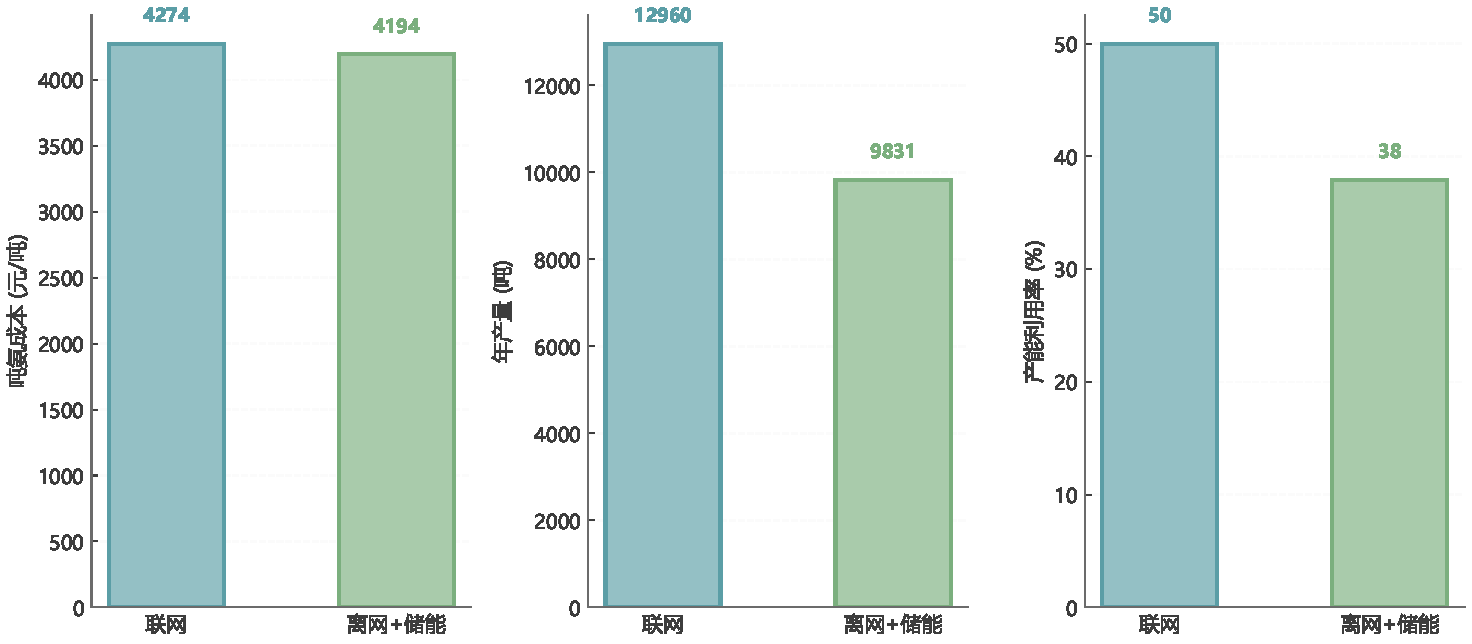
\includegraphics[width=0.85\textwidth,height=0.38\textheight,keepaspectratio]{../figures/fig_q4_economics.pdf}
\caption{离网与联网运行模式经济性对比}\label{fig:q4_economics}
\end{figure}

经济性对比（图\ref{fig:q4_economics}）揭示了两种模式的本质差异。离网模式吨氨成本略低（4194元/吨 vs 4274元/吨，低1.9\%），这是因为离网无购电成本，风光度电成本本身较低。但联网模式的全年产量显著高于离网模式（12960吨 vs 9831吨，高31.8\%），产能利用率也更高（50.0\% vs 37.9\%）。

电网系统支撑的成本价值体现在：联网模式下园区全年净购电成本（购电成本减去售电收入）约为2516万元，这笔费用换来了3129吨的额外产量和12.1个百分点的产能利用率提升。从单位产量角度看，电网支撑的边际价值约为8043元/吨额外产量，高于吨氨成本本身，说明电网提供的调峰备用服务对于维持园区高产能利用率具有不可替代的价值。
